% Optional near-cusp companions to the reference-target root figures.
% Copy these blocks into the desired locations; not automatically included.

\begin{figure}[!ht]
  \centering
  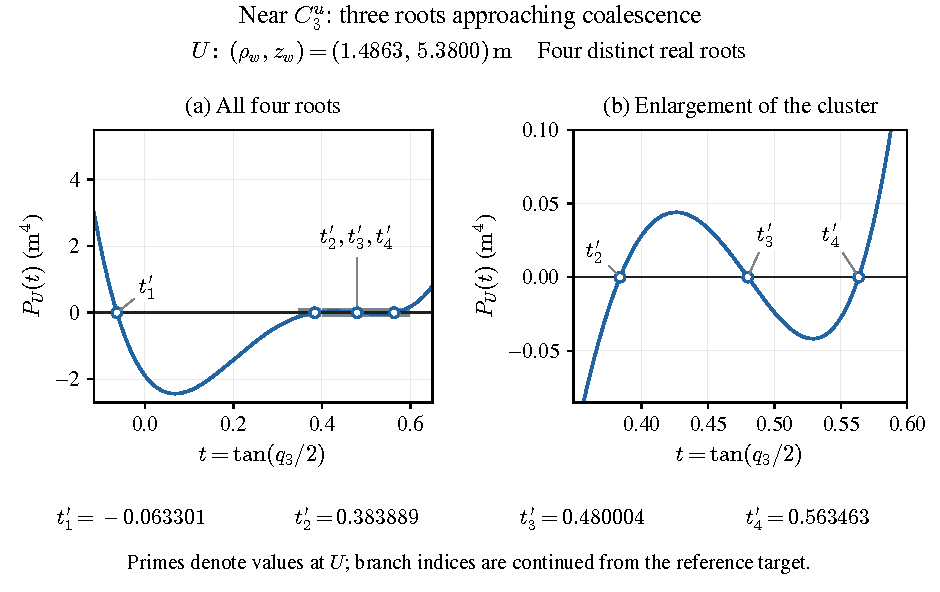
\includegraphics[width=\linewidth]{figures/cusp_quartic.pdf}
  \caption{The arm IK quartic at a target $U$ near the upper cusp $C_3^u$,
  still inside the four-root region. Primes denote root values at $U$;
  the indices are preserved by numerical continuation from the connectivity
  reference target through the four-root region.
  The roots $t_2',t_3',t_4'$ form the cluster that coalesces at $C_3^u$,
  while $t_1'$ remains separated. Panel (b) enlarges the small variations
  around zero that are difficult to distinguish in panel (a).
  All four roots at $U$ are simple.}
  \label{fig:cusp-quartic}
\end{figure}

\begin{figure}[!ht]
  \centering
  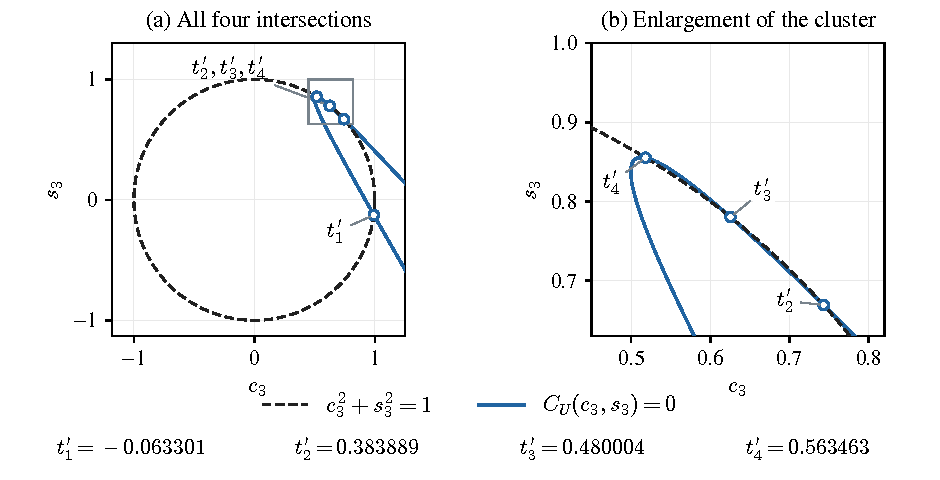
\includegraphics[width=\linewidth]{figures/cusp_circle_conic.pdf}
  \caption{Circle--conic representation of the same near-cusp target $U$.
  The dashed unit circle and solid closure hyperbola meet at four distinct
  points. The enlargement resolves the nearby intersections
  $t_2',t_3',t_4'$, with $t_3'$ between the other two along the circle;
  $t_1'$ is separated from this cluster. At the cusp itself, the three
  intersections coalesce with third-order contact and the associated
  quartic has a triple root. Both panels use equal coordinate scales.}
  \label{fig:cusp-circle-conic}
\end{figure}
